\documentclass{beamer}
\usepackage[latin1]{inputenc}
\usepackage{minted}
\usepackage{graphicx}

\usepackage{etoolbox}
\AtBeginEnvironment{minted}{\singlespacing%
    \fontsize{8}{8}\selectfont}
    
\usetheme{Berlin}

\title[Neural Networks (Part 2)]{Neural Networks (Part 2)}
\author{Matthew Galbraith \& Mitchell Corbett}
\date{April 7, 2015}
\begin{document}

\begin{frame}
    \titlepage
\end{frame}

%%%%%%%%%%%%%%%%%%%%%%%%%%%%%%%%%%%%%%%
%%                MLP                %%
%%%%%%%%%%%%%%%%%%%%%%%%%%%%%%%%%%%%%%%
\section{Multilayer Perceptron Networks}
\begin{frame}
    \frametitle{Multilayer Perceptron Networks:}
            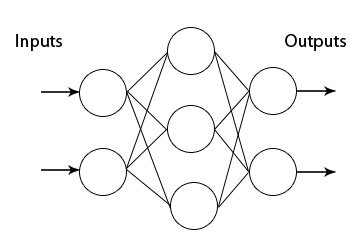
\includegraphics[width=9cm]{mlp.jpg}
\end{frame}

%%%%%%%%%%%%%%%%%%%%%
%%MLP : An overview%%
%%%%%%%%%%%%%%%%%%%%%
\begin{frame}
    \frametitle{Overview}
    \begin{block}{MLP: A type of feed-forward neural network} 
        \begin{itemize}
            \item Network composed of layers of neurons
            \item Each unit (neuron) in the a layer is directly connected to every unit in the following layer, starting from the input layer and ending at the output layer.
            \item The layers between the input and output layer are hidden layers
        \end{itemize}
    \end{block}
\end{frame}

\begin{frame}
    \frametitle{Multilayer Perceptron Networks}
\begin{block}{Overview (Continued)} 
    \begin{itemize}
        \item Whereas a true Perceptron is a binary classifier, Multilayer Perceptron networks are suited for both regression and classification problems.
        \item Clarification: MLP is not one perceptron, (although it's name makes it sound like that) but, a network composed of layers of perceptrons which are free to take any arbitrary activation function. 
    \end{itemize}
\end{block}
\end{frame}

%%%%%%%%%%%%%%%%%%%%%%
%%Formal dfn. of MLP%%
%%%%%%%%%%%%%%%%%%%%%%
\begin{frame}  
    \frametitle{Formal definition of a MLP with one hidden layer}
    \begin{block}{A one-hidden-layer MLP can be represented as a function}
        \item$$f: R^D \rightarrow R^L$$
        \item $D$: size of input vector $x$
        \item $L$: size of the output vector $f(x)$
        \item Continued on chalkboard...
        \end{block}
    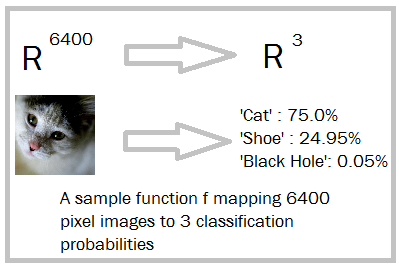
\includegraphics[width=4cm]{sample_f.png}
\end{frame}
%%%%%%%%%%%%%%%%%%%%%%%%%%%%%%%%%%%
%%Universal Approximation Theorem%%
%%%%%%%%%%%%%%%%%%%%%%%%%%%%%%%%%%%
\begin{frame}
    \frametitle{So... What can we model with one-hidden-layer MLPs?}
    \begin{block}{EVERYTHING!}
    \item Well, not quite everything.. But when it comes to continuous functions...
    \item Universal Approximation Theorem
    \item Summarized: A feed-forward network with a single hidden layer containing a finite number of neurons (Sound familiar?) can approximate continuous functions on compact subsets of $R^n$. 
    \item This means simple MLP networks such as the one I've been talking about can be used to model a wide variety of problems!
    \end{block}
\end{frame}
%%%%%%%%%%%%%%%%
%%Training MLP%%
%%%%%%%%%%%%%%%%
\section{Training MLP Networks}
\begin{frame}
    \frametitle{How do we train the Neural Network?}
    \begin{block}{Higher level pseudocode...}
    \begin{itemize}
    \item A typical choice: Uniform random distribution in range $$(\sqrt{-1d},\sqrt{1d})$$
    \item d: dimension of the input
    \item Choice of initial weights is important!
    \end{itemize}
    \end{block}    
\end{frame}

\begin{frame}
    \frametitle{Training the network}
    \begin{block}{How do we train the network?}
    \begin{itemize}
    \item Loss function: typically MSE
    \item Goal: Find weights that minimize the loss function
    \end{itemize}
    \end{block}   
\end{frame}


\section{Updating the weights}
\begin{frame}
    \frametitle{Training the network}
    \begin{block}{High level pseudocode:}
        \item 1. Initialize the weights 
        \item 2. For a number of epochs, we:
        \item 2.1. Forward-pass: We compute the output of the network
        \item 2.1 We compute the loss (MSE) wrt our output
        \item 2.2 Using backpropagation and an optimization method we work backwards to update the weights to minimize the error. 
    \end{block}   
\end{frame}

\begin{frame}[fragile]
\frametitle{Backpropagation}
\begin{minted}{python}
initialize network weights
loop:
forEach training example ex
  #forward-pass:
  prediction = network-output(ex)
  actual = correct-output(ex)
  compute loss at output units
  #backwards propagation:
  compute change in weights from hidden to output layer
  compute change in weights from input to hidden layer
  update network weights
if (stopping criterion satisfied):
    return network
\end{minted}
\end{frame}

\begin{frame}
    \frametitle{Update methods}
    \begin{block}{First order optimization algorithms}
    \item Stochastic Gradient Descent
    \item Gradient Descent with Momentum
    \item Gradient Descent with Nesterov Momentum
    \end{block}
\end{frame}

\begin{frame}[fragile]
    \frametitle{Update methods - SGD}
    \begin{block}{Stochastic Gradient Descent}
    \begin{minted}[linenos]{python}
def sgd(loss, all_params, learning_rate):
    all_grads = theano.grad(loss, all_params)
    updates = []
    for param_i, grad_i in zip(all_params, all_grads):
        updates.append((param_i,
        param_i - learning_rate * grad_i))
    return updates
    \end{minted}
\end{block}

\end{frame}

\begin{frame}[fragile]
    \frametitle{Update methods - Momentum}
    \begin{block}{Gradient Descent with Momentum}
    \begin{minted}[linenos]{python}
def momentum(loss, all_params, learning_rate, momentum=0.9):
    all_grads = theano.grad(loss, all_params)
    updates = []

    for param_i, grad_i in zip(all_params, all_grads):
        mparam_i = theano.shared(np.zeros(param_i.get_value().shape,
                                          dtype=theano.config.floatX),
                                 broadcastable=param_i.broadcastable)
        v = momentum * mparam_i - learning_rate * grad_i
        updates.append((mparam_i, v))
        updates.append((param_i, param_i + v))

    return updates
    \end{minted}
\end{block}
\end{frame}


\begin{frame}[fragile]
    \frametitle{Update methods - Nesterov Momentum}
    \begin{block}{Accelerated Gradient Descent with Nesterov Momentum}
    \begin{minted}[linenos]{python}
# using the alternative formulation of nesterov momentum described at
# https://github.com/lisa-lab/pylearn2/pull/136
# such that the gradient can be evaluated at the current parameters.
def nesterov_momentum(loss, all_params, learning_rate, momentum=0.9):
    all_grads = theano.grad(loss, all_params)
    updates = []

    for param_i, grad_i in zip(all_params, all_grads):
        mparam_i = theano.shared(np.zeros(param_i.get_value().shape,
                                          dtype=theano.config.floatX),
                                 broadcastable=param_i.broadcastable)
        v = momentum * mparam_i - learning_rate * grad_i  # new momemtum
        w = param_i + momentum * v - learning_rate * grad_i  # new param values
        updates.append((mparam_i, v))
        updates.append((param_i, w))

    return updates
\end{minted}
\end{block}
\end{frame}


%%%%%%%%%%%%
%%Analysis%%
%%%%%%%%%%%%
\section{Analysis}


\begin{frame}
    \frametitle{Moving on}
    \begin{block}{MLP applications}
    \item Now that I've introduced MLP Networks..
    \item It's applications time!
    \end{block}
\end{frame}

\begin{frame}
    \frametitle{Moving on}
    \begin{block}{MLP applications}
    \item Now that I've introduced MLP Networks..
    \item It's applications time!
    \end{block}
\end{frame}

\begin{frame}
    \frametitle{Facial Keypoint Recognition}
    \begin{block}{Problem:}
    \item Kaggle competition
    \end{block}
    \begin{block}{Observations:}
    \item 7049 samples of 96x96 dimension images
    \item Up to 15 ($x,y$) pairs of coordinates for each image (Some missing)
    \end{block}
    \begin{block}{Model} We want to model some function $$f : R^{9216} \rightarrow R^{30}$$
    mapping our input image data to 15 pairs of $(x,y)$ coordinates 
    \end{block}
\end{frame}

\begin{frame}[fragile]
\frametitle{}
\begin{block}{Python Packages used}
\begin{minted}{python}
from pandas.io.parsers import read_csv
import numpy as np
import cPickle as pickle
import os.path
import matplotlib.pyplot as plt
import theano
from lasagne import layers
from lasagne.nonlinearities import sigmoid
from lasagne.updates import nesterov_momentum
from nolearn.lasagne import NeuralNet
from sklearn.utils import shuffle

\end{minted}
\end{block}
\end{frame}

\begin{frame}[fragile]
\frametitle{Processing the data}
\begin{block}{Load function courtesy of Daniel Nouri's tutorial}
\begin{minted}{python}
def load(test=False, cols=None, drop_missing=True):
    #...
    df = read_csv(os.path.expanduser(fname))  # load pandas dataframe

    df['Image'] = df['Image'].apply(lambda im: np.fromstring(im, sep=' '))
    if cols:  # get a subset of columns
        df = df[list(cols) + ['Image']]
    if (drop_missing):
        df = df.dropna()  # drop all rows that have missing values
    X = np.vstack(df['Image'].values) / 255.  # scale pixel values to [0, 1]
    X = X.astype(np.float32)

    if not test:  # only FTRAIN has any target columns
        y = df[df.columns[:-1]].values
        y = (y - 48) / 48  # scale target coordinates to [-1, 1]
        X, y = shuffle(X, y, random_state=65539)  # shuffle train data          y = y.astype(np.float32)
    else:
        y = None
    return X, y\end{minted}
\end{block}
\end{frame}

\begin{frame}[fragile]
\frametitle{Processing the data}
\begin{block}{Here's what loads..}
\begin{minted}{python}
>>>X, y = load()
>>>print summary(X,y)
X shape: (2140L, 9216L)
y shape: (2140L, 30L)
X: min, max = (0.0,1.0)
y: min, max = (-0.920286595821,0.996020495892)
Using 30.3589161583% of the provided training data
\end{minted}
\end{block}
\end{frame}
%%%%%%%%%%%%%%%%%%%%%%%%%%%
%%VISUALIZING THE PROBLEM%%
%%%%%%%%%%%%%%%%%%%%%%%%%%%
\begin{frame}[fragile]
\frametitle{Exploring the data}
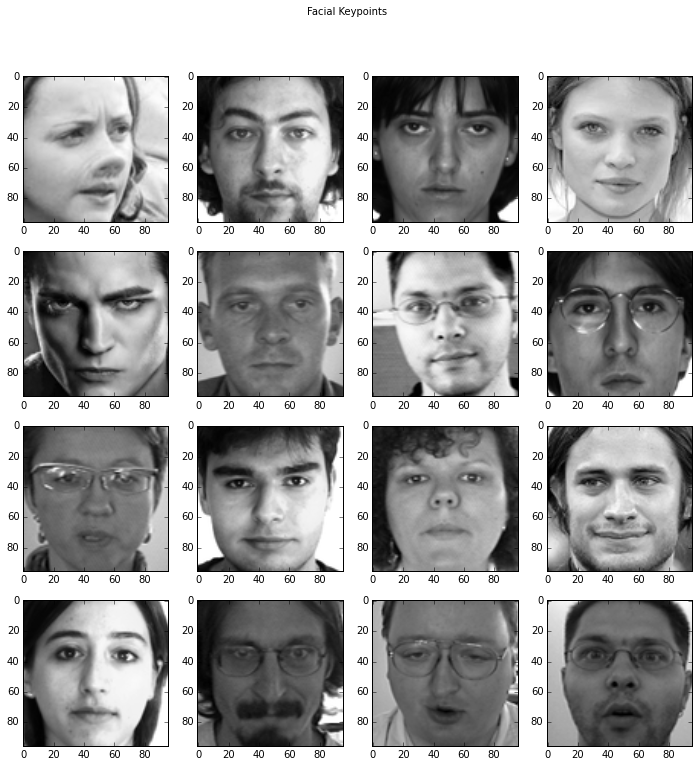
\includegraphics[width=180px]{fk_face.png}
\end{frame}

\begin{frame}[fragile]
\frametitle{Exploring the data}
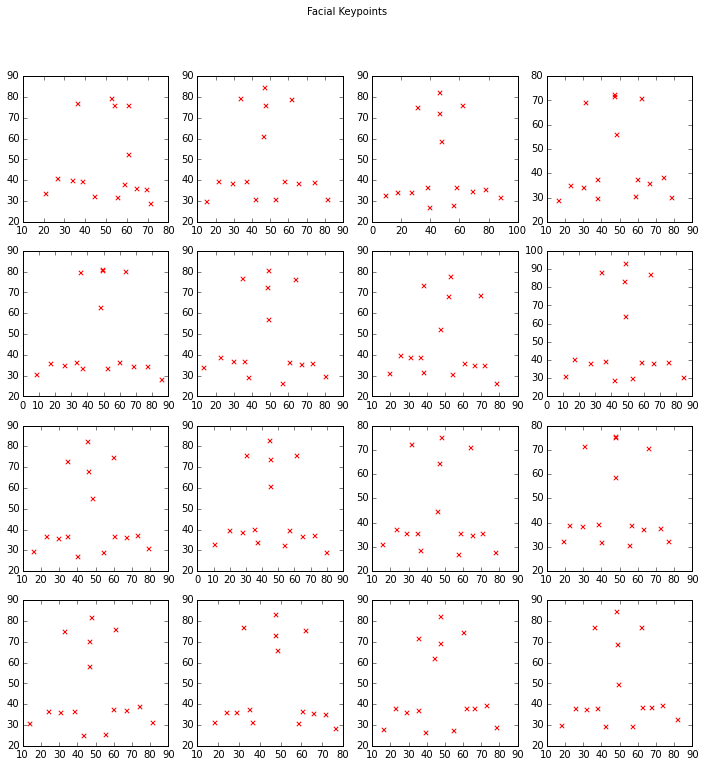
\includegraphics[width=180px]{fk_coord.png}
\end{frame}

\begin{frame}[fragile]
\frametitle{Exploring the data}
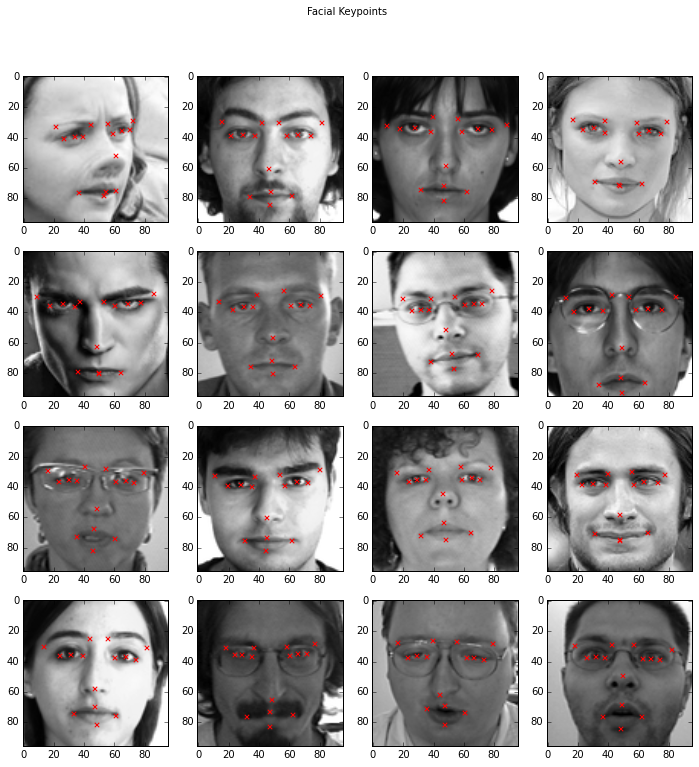
\includegraphics[width=180px]{fk_example.png}
\end{frame}

%%%%%%%%%%%%%%%%%%%
%%MODELLING NNETS%%
%%%%%%%%%%%%%%%%%%%

\begin{frame}[fragile]
\frametitle{Creating NNets in Python}
\begin{block}{Here's the general workflow I followed}
\begin{minted}{python}
#Initialize the network
net = NeuralNet( #layers = ...
                 #more params = ...
                 #max_epochs = n
               )
X, y = load() #Load data
net.fit(X,y) #Train network
#analysis can go here...
X = load(test=false)[0] #Load test data
y_pred = net.predict(X) #Predict
#code to make Kaggle submission goes here...
\end{minted}
\end{block}
\end{frame}

\begin{frame}[fragile]
\frametitle{Using Early Stopping to reduce overfitting}
\begin{minted}[linenos]{python}
class EarlyStopping(object):
    def __init__(self, patience=100):
        self.patience = patience
        self.best_valid = np.inf
        self.best_valid_epoch = 0
        self.best_weights = None

    def __call__(self, nn, train_history):
        current_valid = train_history[-1]['valid_loss']
        current_epoch = train_history[-1]['epoch']
        if current_valid < self.best_valid:
            self.best_valid = current_valid
            self.best_valid_epoch = current_epoch
            self.best_weights = [w.get_value() for w in nn.get_all_params()]
        elif self.best_valid_epoch + self.patience < current_epoch:
            print("Early stopping.")
            print("Best valid loss was {:.6f} at epoch {}.".format(
                self.best_valid, self.best_valid_epoch))
            nn.load_weights_from(self.best_weights)
            raise StopIteration()
\end{minted}
\end{frame}

\begin{frame}[fragile]
\frametitle{Model 1}
\begin{minted}[linenos]{python}
#Neural Network # 1  - A MLP with 1 hidden layer
net1 = NeuralNet(
    layers=[  # three layers: one hidden layer
        ('input', layers.InputLayer),
        ('hidden', layers.DenseLayer),
        ('output', layers.DenseLayer),
        ],
    # layer parameters:
    input_shape=(None, 9216),  # 96x96 input pixels
    hidden_num_units=100,  # number of units in hidden layer
    hidden_nonlinearity=sigmoid,
    output_nonlinearity=None,  # output layer uses identity function
    output_num_units=30,  # 30 target values
    # optimization params
    update=nesterov_momentum,
    update_learning_rate=0.01,
    update_momentum=0.9,
    regression=True, 
    max_epochs=1000,
    on_epoch_finished=[
        EarlyStopping(patience=50)
        ],
    verbose=1 #0 to not print anything
    )
\end{minted}
\end{frame}

\begin{frame}[fragile]
\frametitle{Using gridsearchCV to determine appropriate number of hidden units}
\begin{minted}[linenos]{python}
#paramter grid for gridsearch cv
param_grid = {
'more_params': [{'hidden_num_units': 100}, {'hidden_num_units':150}, {'hidden_num_units': 200},
{'hidden_num_units': 250}, {'hidden_num_units': 300}]
}
 
#find net with best params , and then refit with all data on best net
gs = GridSearchCV(net1, param_grid, cv=2, refit=True, verbose=4)
X,y=load() # Load our data
gs.fit(X,y) #Fit our gridsearchCV object
with open('net1_gridsearch.pickle', 'wb') as f:
    # we serialize the gridsearch model, as it also has the fitted neural network with best hidden unit number:
    pickle.dump(gs, f, -1)
    #if you just want to save the best estimator - ie - the neural network itself - without the gridsearch info:
    #pickle.dump(gs.best_estimator_, f, -1)
\end{minted}
\end{frame}

\begin{frame}[fragile]
\frametitle{Analyzing results of the gridsearchCV}
\begin{minted}[linenos]{python}
>>>#Load the serialized gridsearchCV object which contains our network.
>>>net1_gridsearch = pickle.load(open('./net1_gridsearch.pickle', 'rb'))
>>>#This just shows the params the gridsearch considered when finding the best model
>>>net1_gridsearch.param_grid
{'more_params': [{'hidden_num_units': 100},
  {'hidden_num_units': 150},
  {'hidden_num_units': 200},
  {'hidden_num_units': 250},
  {'hidden_num_units': 300}]}
>>>#Here are the best parameters:
>>>print net1_gridsearch.best_params_
{'more_params': {'hidden_num_units': 100}} 
\end{minted}
\end{frame}

\begin{frame}[fragile]
\frametitle{Grid Search CV results}
\begin{minted}[linenos]{python}
>>>print "The best score (Lowest MSE) was: " + str(net1_gridsearch.best_score_)
>>>print "This translates to a RMSE (Kaggle's evaluation) score of: " + 
str(np.sqrt(net1_gridsearch.best_score_) * 48.)
The best score (Lowest MSE) was: 0.0025870305397
This translates to a RMSE (Kaggle evaluation) score of: 2.44141728581
\end{minted}
\end{frame}

\begin{frame}[fragile]
\frametitle{Analyzing the first Neural Network model}
\begin{minted}[linenos]{python}
#Let's load our neural net from the gridserach object!
>>>net1 = net1_gridsearch.best_estimator_
>>>net1
NeuralNet(X_tensor_type=<function matrix at 0x...>,
     batch_iterator_test=<nolearn.lasagne.BatchIterator object at 0x...>,
     batch_iterator_train=<nolearn.lasagne.BatchIterator object at 0x...>,
     eval_size=0.2,
     hidden_nonlinearity=<theano.tensor.elemwise.Elemwise object at 0x...>,
     hidden_num_units=100, input_shape=(None, 9216),
     layers=[('input', <class 'lasagne.layers.input.InputLayer'>),
     ('hidden', <class 'lasagne.layers.dense.DenseLayer'>),
     ('output', <class 'lasagne.layers.dense.DenseLayer'>)],
     
     loss=<function mse at 0x...>, max_epochs=1000,
     more_params={'hidden_num_units': 100},
     on_epoch_finished=[<__main__.EarlyStopping object at 0x...>],
     on_training_finished=(), output_nonlinearity=None,
     output_num_units=30, regression=True,
     update=<function nesterov_momentum at 0x...>,
     update_learning_rate=0.01, update_momentum=0.9,
     use_label_encoder=False, verbose=1,
     y_tensor_type=TensorType(float32, matrix))
\end{minted}
\end{frame}


\begin{frame}[fragile]
\frametitle{Model 1 - Learning Curve}
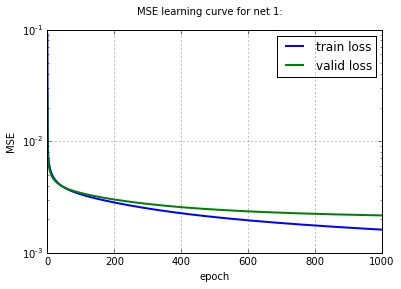
\includegraphics[width=310px,height=200px]{net1_learningMSE.png}
\end{frame}

\begin{frame}[fragile]
\frametitle{Model 1 - Learning Curve}
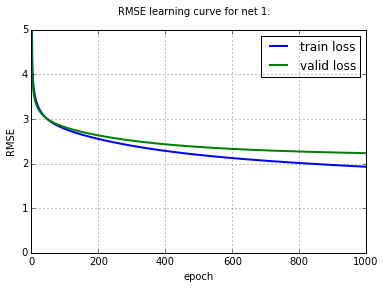
\includegraphics[width=310px,height=200px]{net1_learningRMSE.png}
\end{frame}

\begin{frame}[fragile]
\frametitle{Plotting a sample prediction}
Taking a sample face (from the training set), here are predicted coordinates:
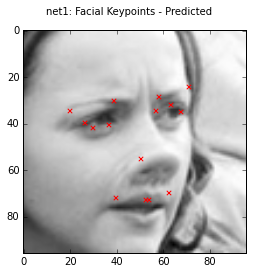
\includegraphics[width=150px,height=150px]{net1_sampleprediction_ontrain_predicted.png}
\end{frame}

\begin{frame}[fragile]
\frametitle{Plotting a sample prediction --pt.2}
Taking a sample face (from the training set), here are the actual coordinates:
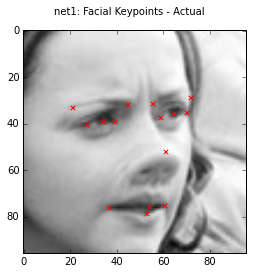
\includegraphics[width=150px,height=150px]{net1_sampleprediction_ontrain_actual.png}
\end{frame}

\begin{frame}[fragile]
\frametitle{Kaggle submission --pt.1}
Here's a plot of predicted keypoints for a Kaggle test sample:
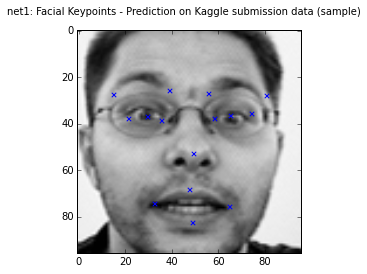
\includegraphics[width=150px,height=150px]{net1_test_prediction.png}
\end{frame}

\begin{frame}[fragile]
\frametitle{Kaggle submission --pt.2}
\begin{block}{Submitting to kaggle!}
\item Not as simple as predicting and writing to csv...
\item Submission only wants specific coordinates from specific images in the test set
\item Need to filter our predictions by the coordinates Kaggle wants
\end{block}
\end{frame}


\begin{frame}[fragile]
\frametitle{Kaggle submission --pt.3}
\begin{block}{Submission made!}
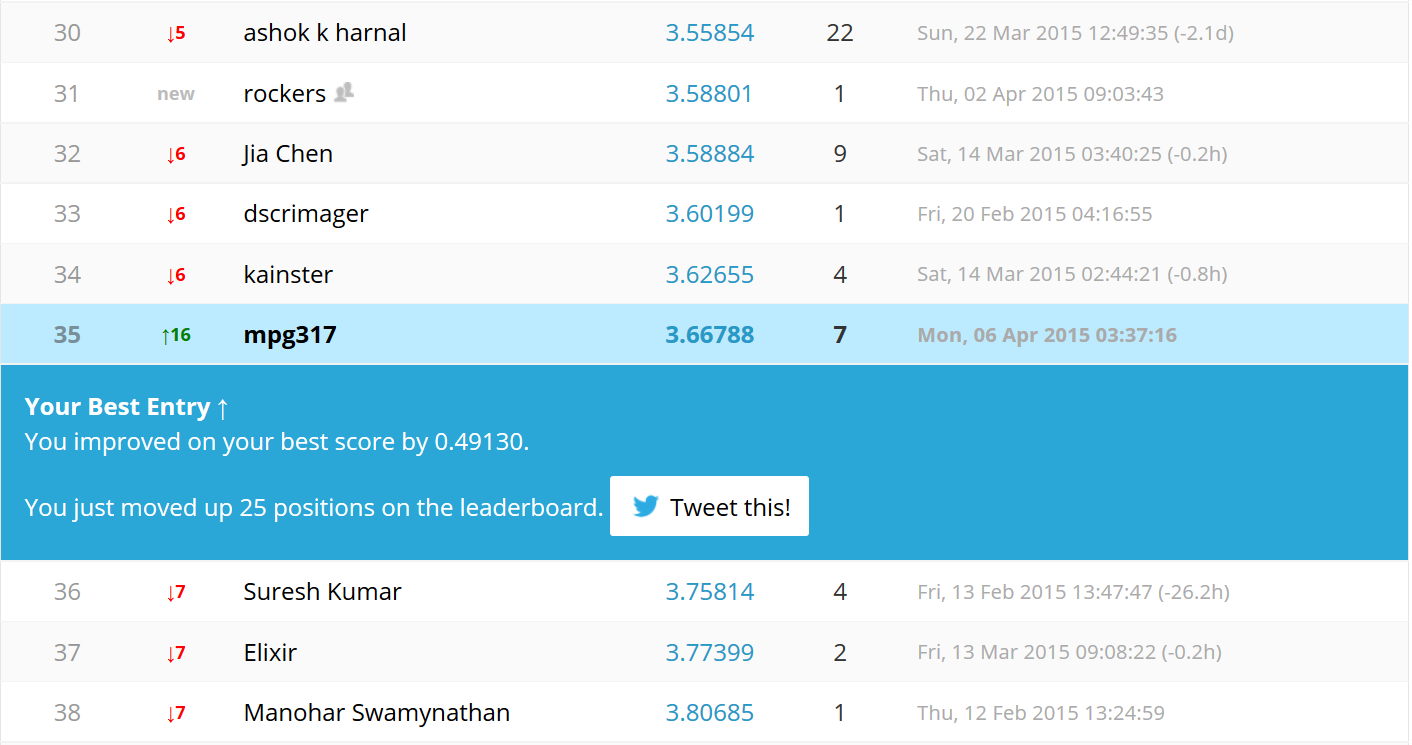
\includegraphics[width=280px,height=150px]{net1_kaggle_submission_score.png}
\end{block}
\end{frame}

\begin{minted}[linenos]{python}

\end{minted}
\end{frame}
\begin{frame}[fragile]
\frametitle{Title}
\begin{minted}[linenos]{python}

\end{minted}
\end{frame}
\begin{frame}[fragile]
\frametitle{Title}
\begin{minted}[linenos]{python}

\end{minted}
\end{frame}


\end{document}